\section{Db2 Graph}
\label{chap:db2graph}

Im Rahmen dieses Kapitels wird IBM Db2 Graph genauer beschrieben. Im Zuge dessen werden der Ansatz, der Aufbau, die Funktionsweise und die bereits bekannten Einschränkungen  von Db2 Graph erläutert. Außerdem werden die verschiedenen Optimierungsmechanismen von Db2 Graph erörtert und die Unterschiede zwischen den Versionen von Db2 Graph behandelt,  die im Rahmen der Arbeit eine Rolle spielen. Abschließend werden die wichtigsten Details zu Db2 Graph nochmals kurz zusammengefasst.

\subsection{Ansatz}
\label{db2graph:ansatz}
Db2 Graph wurde mit dem Ziel entwickelt, Informationen mittels Graph-Queries aus einer relationalen Db2 Datenbank abfragen zu können \cite{vldb_tian, sigmod_tian}. So wurde Db2 Graph als eine Art Graph-Erweiterung für Db2 konzipiert. Der Einsatz von Db2 Graph setzt dabei eine aktive Instanz von Db2 voraus \cite{vldb_tian, sigmod_tian}. Diese hält hierbei die Informationen, auf die Db2 Graph Zugriff hat, in relationaler Form \cite{vldb_tian, sigmod_tian}. Dabei müssen die Daten nicht für die Einbindung in Db2 Graph angepasst oder umformatiert werden \cite{vldb_tian, sigmod_tian}.

\begin{figure}[ht]
    \centering
    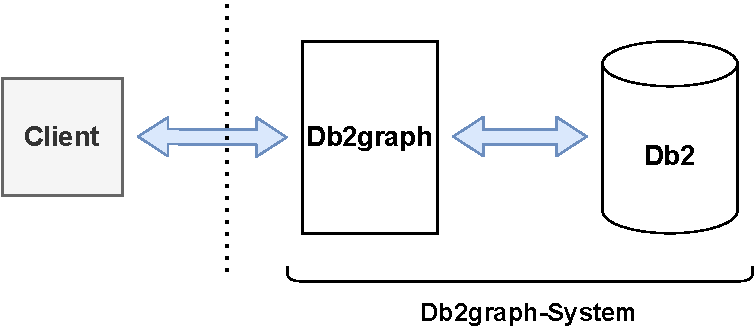
\includegraphics[width=\textwidth]{images/db2graph_system.pdf}
    \vspace{0.1em}
    \caption{Struktur Db2 Graph-System}
    \label{fig:db2graph_system}
\end{figure}

Wie in \autoref{fig:db2graph_system} erkennbar, fungiert Db2 Graph aus architektonischer Sicht als eine Art Proxy-Anwendung für Db2. Dabei übersetzt sie die von einem Client gesendeten Gremlin-Graph-Queries in SQL-An\-wei\-sung\-en \cite{vldb_tian, sigmod_tian}. Diese werden anschließend an eine Db2 Instanz weitergeleitet \cite{vldb_tian, sigmod_tian}. 

Db2 Graph und Db2 erfüllen somit gemeinsam die Rolle einer Read-Only-Graph\-daten\-bank. Db2 Graph vereint dabei Elemente von Graph- und relationalen Datenbanksystemen. So ist es möglich Graph-Anfragen an ein System zu stellen, das die Daten in relationaler Form speichert \cite{vldb_tian, sigmod_tian}. Dadurch bringt Db2 Graph das Abfragen von Elementen einer Graphstruktur mit einer relationalen Datenhaltung zusammen. 

\subsection{Aufbau}
Wie in \autoref{fig:db2graph_aufbau} beschrieben, handelt es sich bei Db2 Graph um eine modular aufgebaute Anwendung. Die Anwendung besteht dabei aus fünf größeren Komponenten. Diese fünf Komponenten übernehmen dabei die folgenden Rollen und Aufgaben: 

\begin{itemize}
    \item \textit{TinkerPop-Stack}\\Stellt das Grundgerüst für Db2 Graph dar. Er parst eingehende Gremlin-Queries und erstellt auf Basis dessen einen Query-Plan bzw. Abfrage-Plan \cite{vldb_tian}. Dabei interagiert er über API-Aufrufe mit den anderen Modulen \cite{vldb_tian}.
    \item \textit{Topology}\\Beinhaltet die Funktionalität für das Mapping von relationalen Tabellen auf eine Graph-Struktur \cite{vldb_tian, sigmod_tian}.
    \item \textit{Graph Structure}\\Hierbei handelt es sich um eine eigene Implementierung einer Graph-Struktur, auf deren Basis TinkerPop arbeitet \cite{vldb_tian}. Eine Implementierung dieser Struktur wird benötigt, um den vom TinkerPop-Stack erstellten Query-Plan durchzuführen \cite{sigmod_tian}. 
    \item \textit{SQL-Dialect}\\Diese Komponente stellt die Funktionalität für die Erzeugung von Db2-kompatiblen SQL-Anweisungen bereit \cite{sigmod_tian}.
    \item \textit{Traversal-Strategy}\\Dieses Modul stellt dem TinkerPop-Stack optimierte Traversal-Strategies zur Verfügung. Diese werden eingesetzt, um einen vom TinkerPop-Stack aufgestellten Query-Plan zu optimieren, bevor dieser ausgeführt wird \cite{sigmod_tian}.  
\end{itemize}

Der TinkerPop-Stack stellt somit den Kern von Db2 Graph dar. Die Topology-, Graph-Structure- und SQL-Dialect-Komponente abstrahieren die Db2 Graph spezifische Funktionalität, auf die der TinkerPop-Stack zugreifen kann \cite{sigmod_tian}. Zusätzlich dazu stellt das Traversal-Strategy-Modul dem TinkerPop-Stack, optimierte Traversal-Strategies bereit \cite{sigmod_tian}. Diese helfen dem TinkerPop-Stack dabei die Performance von Query-Plans zu verbessern \cite{sigmod_tian}.  

\begin{figure}[ht]
    \centering
    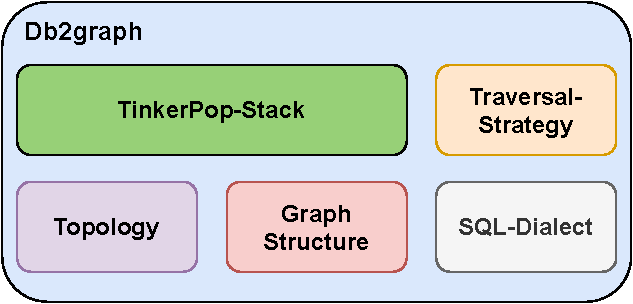
\includegraphics[width=\textwidth]{images/db2graph_components.pdf}
    \caption{Aufbau von Db2 Graph}
    \label{fig:db2graph_aufbau}
    \vspace{0.5em}
    \textit{Der hier gezeigter Aufbau von Db2 Graph   orientiert sich an der Beschreibung der System-Architektur in} \cite{vldb_tian} \textit{und} \cite{sigmod_tian}\textit{.}
\end{figure}

\subsection{Funktionsweise}
\label{db2graph:funktionsweise}
Um die Funktionsweise von Db2 Graph genauer zu erläutern, wird in diesem Abschnitt die Funktionsweise aus verschiedenen Perspektiven erläutert. Im Rahmen der ersten externen Perspektive wird detailliert darauf eingegangen, wie die Anfrage eines Clients in Db2 Graph und Db2 verarbeitet wird. Der Fokus liegt hierbei auf der Kommunikation zwischen den Anwendungen. Bei der zweiten Perspektive handelt es sich hingegen um die Db2 Graph interne Perspektive. Im Zuge dessen wird beschrieben, wie eine Gremlin-Abfrage von einer Db2 Graph-Anwendung intern verarbeitet wird. 

Im Anschluss an diese beiden Perspektiven wird der Begriff und die Funktionsweise des Mapping in Db2 Graph genauer erläutert. Schließlich spielen die damit in Verbindung stehenden Topologie-Informationen eine wichtige Rolle für die Verarbeitung von Anfragen.

\subsubsection{Extern}
Im Rahmen dieses Unterabschnitts wird darauf eingegangen, wie die Verarbeitung einer Anfrage (Gremlin-Query) im Kontext der voneinander entkoppelten Bestandteile Client(-Anwendung), Db2 Graph und Db2 erfolgt. Der Ablauf der  Verarbeitung kann dabei in die folgenden Schritte unterteilt werden: 
\begin{enumerate}
    \item Ein Client sendet eine Gremlin-Query an Db2 Graph. 
    \item Db2 Graph wandelt die Gremlin-Query in SQL-Statements um. 
    \item Db2 Graph sendet die erzeugten SQL-Statements an Db2.
    \item Db2 verarbeitet die SQL-Statements.
    \item Db2 leitet die Ergebnisse an Db2 Graph weiter.
    \item Db2 Graph bereitet die von Db2 empfangen Ergebnisse für den Client auf. 
    \item Db2 Graph übermittelt die Ergebnisse an den Client.
\end{enumerate}

Die soeben beschriebenen Schritte des Ablaufs können dabei den in der \autoref{fig:db2graph_processing} aufgeführten Schritten zugeordnet werden. Die in \autoref{fig:db2graph_processing} als grün gekennzeichnet Pfeile markieren dabei die Schritte, in den die Anfrage in Form einer Gremlin-Query oder SQL-Anfragen weitergeleitet oder verarbeitet wird. Die Pfeile, welche in \autoref{fig:db2graph_processing} lila gefärbt sind, heben die Schritte hervor, in denen die abgefragten Daten transformiert oder weitergeleitet werden.

\begin{figure}[ht]
    \centering
    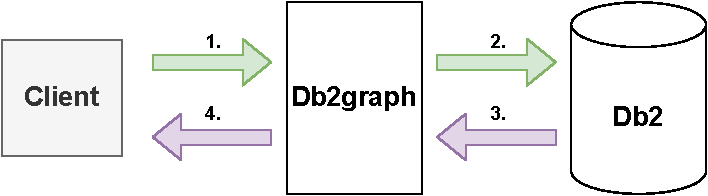
\includegraphics[width=\textwidth]{images/db2graph_processing.pdf}
    \caption{Externe Verarbeitung Db2 Graph}
    \label{fig:db2graph_processing}
    \vspace{1em}
    \textit{Die dargestellten Abläufe basieren hierbei unter anderem auf den in} \cite{vldb_tian} \textit{und} \cite{sigmod_tian} \textit{beschrieben Abläufen der Verarbeitung. Darüber hinaus wurden auch einige kleinere Details von} \cite{tinkerpop_2020} \textit{bezogen.} 
\end{figure}

\subsubsection{Intern}
Im Rahmen dieses Unterabschnitts wird dargelegt, wie eine von Db2 Graph empfangene Gremlin-Query intern verarbeitet wird. Der Ablauf kann dabei in die folgenden Schritte gegliedert werden: 

\begin{enumerate}
    \item Ein Client baut eine Verbindung auf und sendet eine Gremlin-Query Db2 Graph.
    \item Der TinkerPop-Stack lädt Informationen über die Beschaffenheit des in der Gremlin-Query enthaltenen Zielgraphen aus Topology-Komponente \cite{vldb_tian,sigmod_tian, yt_tian}.
    \item Der TinkerPop-Stack erstellt auf Basis der Gremlin-Query und der Topologie-Informationen einen logischen Query-Plan \cite{vldb_tian,sigmod_tian, yt_tian}. 
    \item Der TinkerPop-Stack nutzt das Traversal-Strategy-Modul, um den logischen Query-Plan zu optimieren \cite{vldb_tian,sigmod_tian, yt_tian}. Wie und welche Optimierungen an dieser Stelle angewandt werden, werden in \nameref{db2graph:optimierung} unter \autoref{subsubsec:data_independent_optimizations} genauer erläutert.
    \item Der TinkerPop-Stack wandelt den optimierten logischen Query-Plan in einen physikalischen Query-Plan um \cite{vldb_tian,sigmod_tian, yt_tian}. 
    \item Bei der Ausführung der Steps im physikalischen Query-Plan werden API-Zugriffe auf die Graph-Structure-Komponente durchgeführt \cite{vldb_tian,sigmod_tian, yt_tian}. Um die für diese Zugriffe benötigten Informationen zu beschaffen, lädt die Graph-Structure-Komponente Informationen aus dem Topology-Modul und nutzt die SQL-Dialect-Komponente für die Erzeugung von SQL-Statements \cite{vldb_tian,sigmod_tian, yt_tian}. Bei diesem Schritt können ebenfalls Optimierung angewandt werden. Diese werden in \autoref{db2graph:optimierung} unter \nameref{subsubsec:data_dependent_optimizations} aufgeführt und beschrieben.
    \item Die von der Graph-Structure-Komponente erzeugten SQL-Statements werden an eine Db2 Instanz gesendet und von dieser verarbeitet \cite{vldb_tian,sigmod_tian, yt_tian}.
    \item Die daraufhin von Db2 erhalten und zurückgesendeten Ergebnisse werden von der Graph-Structure-Komponente verarbeitet \cite{yt_tian}. 
    \item Die Graph-Komponente nutzt die verarbeiteten Ergebnisse, um die API-Aufrufe des TinkerPop-Stacks zu beantworten \cite{vldb_tian,sigmod_tian, yt_tian}.
    \item Nach der Durchführung des physikalischen Query-Plans -- inklusive der API-Aufrufe auf die Graph-Structure-Komponente -- werden die Ergebnisse vom TinkerPop-Stack an den Client übermittelt \cite{vldb_tian,sigmod_tian, yt_tian}.
\end{enumerate}

Die in der zuvor aufgelisteten Schritten 1. bis 7. wurden dabei in der \autoref{fig:db2graph_intern_processing} visuell dargestellt.

\begin{figure}[ht]
    \centering
    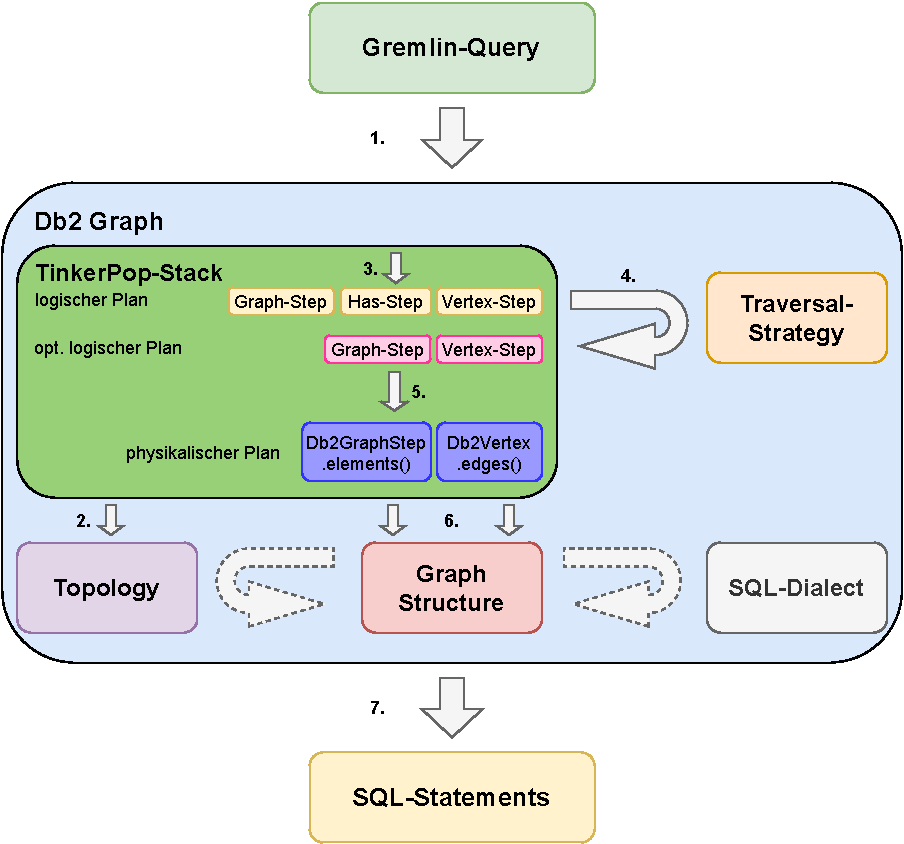
\includegraphics[width=\textwidth]{images/db2graph_intern_processing.pdf}
    \caption{Interne Verarbeitung Db2 Graph}
    \label{fig:db2graph_intern_processing}
    \vspace{1em}
    \textit{Die in der Abbildung dargestellten Abläufe basieren auf den in} \cite{yt_tian}\textit{,} \cite{vldb_tian} \textit{und} \cite{sigmod_tian} \textit{beschrieben Abläufen.} 
\end{figure}

\subsubsection{Mapping}
Bei dem sogenannten Mapping handelt es sich um den Db2 Graph-internen Prozess beziehungsweise Technik, bei dem eine Graph-Struktur relationalen Daten überge\-stülpt wird beziehungsweise diese überlagert. Der Prozess kann auch als Graph-Overlaying bezeichnet werden. Vereinfacht ausgedrückt, handelt es sich dabei um die Spezifikation der Topologie des von Db2 Graph abgebildeten Graphen. In dieser Spezifikation wird festgelegt, welche relationalen Tabellen und Spalten auf welche Graph-Elemente (Knoten und Kanten) gemappt werden. 

Für die Bereitstellung und Verarbeitung des Mapping in Db2 Graph ist hierbei die Topology-Komponente zuständig. Das Mapping wird dabei in einer als Graph-Overlay-Konfiguration bezeichneten Datei festgehalten.  

Um das Mapping von relationalen auf Graph-Strukturen durchzuführen, werden den relationalen Tabellen verschiedene Rollen zugewiesen. Dabei sind die zwei folgenden Rollen verfügbar:
\begin{itemize}
    \item \textit{Vertex-Tabelle}\\Die Zeilen einer Tabelle werden als Knoten auf einen Graph gemappt \cite{sigmod_tian, yt_tian}.
    \item \textit{Edge-Tabelle}\\Die Zeilen dieser Tabelle werden als Kanten auf einen Graph gemappt \cite{sigmod_tian, yt_tian}.
\end{itemize}

% TODO Basti würde hier ein Schaubild gefallen

Um Verbindungen zwischen Kanten und Knoten herzustellen verfügt eine Vertex-Tabelle über eine Vertex-ID (\texttt{vid}). Diese \texttt{vid} kann als eine Art Primärschlüssel betrachtet werden. Die \texttt{vid} setzt sich dabei aus einer oder mehreren Spalten einer relationalen Tabelle und einem Prefix zusammen \cite{sigmod_tian, yt_tian}, siehe \texttt{prefix} und \texttt{id\_cols} Zeile 5-6 in \autoref{src:mapping_example}. Ihr Zweck ist es dabei, immer einen einzigen bestimmten Knoten über den Wert den \texttt{vid} identifizieren zu können \cite{sigmod_tian, yt_tian}. 

Auf Basis dieser \texttt{vid} -- Zeile 4 - 7 \autoref{src:mapping_example} -- setzt beim Mapping auch die Edge-Tabelle auf. So ist es notwendig den Quell- und Ziel-Knoten einer Kante in der Edge-Tabelle anzugeben. Dafür muss bei der Referenzierung eines Quell-Knoten in der Graph-Overlay-Konfiguration die Tabellen-ID der Vertex-Tabelle angegeben werden, die den Quell-Knoten enthält. Siehe \texttt{table\_id} und \texttt{src\_v\_tables} Zeile 8 und 23 in \autoref{src:mapping_example}. Zusätzlich dazu müssen auch die Spalten in der Edge-Tabelle spezifiziert werden, anhand derer eine Zeile der Vertex-Tabelle referenziert wird. Siehe \texttt{src\_v\_cols} in Zeile 21 \autoref{src:mapping_example}. Die Referenzierung eines Ziel-Knotens funktioniert dabei ähnlich. Der einzige Unterschied stellt dabei die Verwendung der Felder \texttt{dst\_v\_cols} und \texttt{dst\_v\_tables} in Zeile 22 und 24 des \autoref{src:mapping_example} dar, statt \texttt{src\_v\_tables} und \texttt{src\_v\_cols}.

Wie im \autoref{src:mapping_example} erkennbar ist, lässt die Konfiguration auch weitere Anpassungen bezüglich des Mappings und der Graph-Topologie zu. So ist es beispielsweise möglich die Labels für Knoten und Kanten auf Basis einer Vertex-Tabelle oder Edge-Tabelle zu definieren, siehe Zeile 15 und 43 \autoref{src:mapping_example}. Der Kern des Mappings spielt sich dabei aber wie zuvor beschrieben auf Basis der Parameter \texttt{vid}, \texttt{table\_id}, \texttt{src\_v\_cols}, \texttt{dst\_v\_cols} sowie \texttt{dst\_v\_tables} und \texttt{src\_v\_tables} ab. Diese Werte bestimmten, wie die relationalen Daten auf einem Graph abgebildet werden.

\begin{lstlisting}[caption={Beispiel Auschnitt Mapping Konfiguration},language=json,label=src:mapping_example]
{
    "v_tables": [
            {
            "vid": {
                "prefix": "LINKDB0.NODETABLE",
                "id_cols": ["ID"]
            },
            "table_id": "LINKDB0.NODETABLE",
            "table": {
                "schema_name": "LINKDB0",
                "table_name": "NODETABLE"
            },
            "label": {
                "fixed_label": true,
                "label": "NODETABLE"
            }
        }
    ],
    "e_tables": [
        {
            "src_v_cols": ["ID1"],
            "dst_v_cols": ["ID2"],
            "src_v_tables": ["LINKDB0.NODETABLE"],
            "dst_v_tables": ["LINKDB0.NODETABLE"],
            "eid": {
                "implicit_id": false,
                "id": {
                    "prefix": "LINKDB0.LINKTABLE",
                    "id_cols": [
                        "LINK_TYPE",
                        "ID1",
                        "ID2"
                    ]
                }
            },
            "table_id": "LINKDB0.LINKTABLE",
            "table": {
                "schema_name": "LINKDB0",
                "table_name": "LINKTABLE"
            },
            "label": {
                "fixed_label": true,
                "label": "LINKTABLE"
            }
        }
    ]
}
\end{lstlisting}

Abschließend zum Thema Mapping sollte auch darauf hingewiesen werden, dass nicht alle Tabellen einer Datenbank oder eines bestimmten Schemas auf einen Graphen gemappt werden müssen. Es ist vollkommen legitim relationalen Tabellen keine Rolle als Vertex-Tabelle oder Edge-Tabelle zuzuweisen. Besonders, wenn die Daten im Kontext des Graphen nicht benötigt werden. 

\subsection{Fähigkeiten \& Einschränkungen}
Im Rahmen dieses Kapitels werden die bekannten Fähigkeiten und Einschränkungen von Db2 Graph kurz zusammengefasst. Dies ist hier von besonderem Interesse, da es sich bei Db2 Graph in Kombination mit Db2 um eine Art hybrides Datenbankmanagementsystem handelt. Auf die besonderen Eigenschaften des Systems, die sich aus der Verbindung von relationalem und Graph-Datenbanksystem ergeben, wird hier ebenfalls eingegangen. 

Db2 Graph verfügt über die folgenden Fähigkeiten und Einschränkungen:

\begin{itemize}
    \item \textit{Read-Only-Queries}\\
    Db2 Graph verfügt über eine read-only Implementierung von Apache TinkerPop, daher ist es dazu in der Lage nahe zu alle read-only Gremlin-Queries zu verarbeiten \cite{ibm_docs_limitiations}. Umgekehrt bedeutet dies allerdings auch, dass Db2 Graph nicht fähig ist schreibende Gremlin-Queries zu verarbeiten.
    \item \textit{Optimierung}\\
    Db2 Graph verfügt über mehrere Mechanismen um die Verarbeitung von empfangen Gremlin-Queries zu optimieren, mehr dazu in \autoref{db2graph:optimierung}.
    \item \textit{Datentypen}\\
    Von Db2 Graph werden nur Datentypen unterstützt, die auch in Db2 vorhanden sind \cite{ibm_docs_limitiations}. Das bedeutet, das nur diese Datentypen als Property-Type eines Knotens oder einer Kante eingesetzt werden können \cite{ibm_docs_limitiations}. Somit ist es auch nicht möglich verschachtelte Datentypen -- wie z.B. in Neo4j -- als Property-Type zu nutzen. Schließlich werden diese nicht von Db2 Graph unterstützt.
    \item \textit{Festes Schema}\\
    Daten die von Db2 Graph abgefragt werden können, verfügen über ein festes Schema. Diese ergibt sich daraus, dass die Daten in einer Db2 Instanz (relational) gehalten und gespeichert werden \cite{sigmod_tian,vldb_tian,yt_tian}.
    \item \textit{Gremlin-Graph-API}\\
    Die Gremlin-Graph-API wird von Db2 Graph nicht unterstützt \cite{ibm_docs_limitiations}. Mehr dazu in !TODO REF Erweiterbarkeit.
\end{itemize}

\subsection{Optimierung}
\label{db2graph:optimierung}

Im Kontext dieses Unterabschnitts wird eine Übersicht über die Optimierungsmechanismen von Db2 Graph geben. Hierfür stützt sich diese Arbeit, auf die in \cite{sigmod_tian} beschrieben Optimierungstechniken. Auch die Unterteilung der Mechanismen in die Kategorien Data-Independent Optimizations und Data-Dependent Optimizations werden dabei aus \cite{sigmod_tian} übernommen. Zum Schluss werden noch Optimierungsmechanismen angesprochen, die nach dem Paper \cite{sigmod_tian} hinzugekommen sind und in \cite{ibm_docs_optimize} beschrieben werden. Dabei handelt es sich auch um Optimierungen, die nicht von beiden im Rahmen dieser Arbeit untersuchten Db2 Graph Versionen unterstützt werden. 

Diese Optimierungen sind notwendig, da ohne sie:

\begin{itemize}
    \item bei jeder Anfrage alle Vertex- oder Edge-Tabellen abgefragt werden würden, 
    \item von Db2 Graph von Db2 obsolete Datenabfragen würde oder 
    \item Db2 Graph selbst die Aggregation oder das Filtern von Ergebnismengen durchführen müsste.
\end{itemize}

\subsubsection{Data-Independent Optimizations}
\label{subsubsec:data_independent_optimizations}
Bei Data-Independent Optimizations handelt es sich um Optimierungstechniken, die Teil des Traversal-Strategy-Moduls sind \cite{sigmod_tian}. Sie werden eingesetzt, um einen logischen Query-Plan zu optimieren. Ihr Anwendung erfolgt dann, wenn bestimmte Muster erkannt werden. Optimierungen die in diese Kategorie fallen, können dem Schritt 4. in \autoref{fig:db2graph_intern_processing} zugeordnet werden. 

In die Kategorie Data-Independent Optimizations fallen dabei die folgenden Techniken: 

\begin{itemize}
    \item \textit{Predicate Pushdown with Filter Steps}\\
    Diese Optimierung wird angewendet, wenn ein Graph-Structure-Access-Step wie \texttt{g.V()} oder \texttt{g.E()} von einem oder mehreren Filter-Steps gefolgt wird \cite{sigmod_tian}. Dabei werden alle Filter-Steps in den Graph-Structure-Access-Step als Predicats eingebettet \cite{sigmod_tian}. Das Endprodukt der Optimierung stellt hierbei ein neuer Graph-Step dar, welcher auf Basis des Graph-Structure-Access-Steps und der Filter-Steps erstellt wurde \cite{sigmod_tian}. 
    
    Um die Funktionsweise der Optimierung zu verdeutlichen, kann die Gremlin-Query \code{g.V().has(``id", 1).has(``type'', ``A'')} herangezogen werden. Bei der Optimierung des aus dieser Query resultierenden Query-Plans, werden der Graph-Structure-Access-Step und die Has-Steps in einen einzigen neuen Graph-Step umgewandelt. So wird bei der Ausführung dieses neuen Graph-Steps der SQL-Code \code{SELECT * FROM VertexTable WHERE id = 1 AND type = ``A''} erzeugt. An diesem lässt sich erkennen, dass die Has-Steps als Teil einer \code{WHERE}-Bedingung in die Abfrage eingebettet wurden.

    Infolge dieser Optimierung erhält Db2 Graph von Db2  kleinere Ergebnismenge.

    \item \textit{Projection Pushdown with Properties Steps}\\
    Diese Optimierung greift, wenn Db2 Graph eine Gremlin-Query verarbeitet, in der bestimmte Properties von Knoten oder Kanten abgefragt werden \cite{sigmod_tian}. Dabei werden die abgefragten Properties in die Projektion eines vorausgegangenen Gremlin-Steps eingebettet. Auf diese Weise erhält Db2 Graph eine kleinere Ergebnismenge von Db2. Diese umfasst dabei lediglich die benötigten Informationen. Darüber hinaus gilt es zu beachten, dass neben den angegeben Properties, auch die \texttt{id\_cols} -- siehe Zeile 6 und 28 in \autoref{src:mapping_example} -- als Informationen von Db2 Graph benötigt werden. 

    Ein gutes Beispiel dafür, wie die Optimierung durchgeführt wird, bietet die Gremlin-Query \code{g.V().values(``data'', ``time'')}. Die Projektion aus dem Values-Step wird dabei zusammen mit den \texttt{id\_cols} in den Graph-Structure-Access-Step integriert. So wird der neue optimierte Graph-Step später in die folgende SQL-Anweisungen übersetzt: \code{SELECT id, type,
    data, time FROM VertexTable}. Ohne die Optimierung wäre der Graph-Step so übersetzt worden: \code{SELECT * FROM VertexTable}.

    \item \textit{Aggregate Pushdown with Aggregation Steps}\\
    Wenn ein Graph-Structure-Access-Step von einem Aggregations-Step, wie \texttt{count}, \texttt{mean}, \texttt{min}, \texttt{max} und \texttt{sum}, gefolgt wird, setzt die Optimierung ein \cite{sigmod_tian}. Dabei wird die Aggregation in den Graph-Structure-Access-Step eingebettet \cite{sigmod_tian}. Dadurch erhält Db2 Graph bei der Ausführung des neuen Graph-Steps ausschließlich die bereits von Db2 aggregierten Ergebnisse.
    
    Die Gremlin-Query \code{g.V().count()} würde dabei zu einem einzelnen Graph-Step optimiert \cite{sigmod_tian}. Dieser ließe sich dann später bei der Ausführung in den SQL-Code \code{SELECT COUNT(*) FROM VertexTable} übersetzen \cite{sigmod_tian}.

    \item \textit{GraphStep::VertexStep Mutation}\\
    Diese Optimierung wird angewandt, wenn ein Graph-Structure-Access-Step Vertexes abfragt und von einem Vertex-Step \cite{sigmod_tian}. Die Optimierung zielt dabei darauf ab unnötige SQL-Abfragen zu vermeiden \cite{sigmod_tian}. 

    Die Optimierung lässt sich dabei verständlich anhand der Gremlin-Query \code{g.V(ids).outE()} \cite{sigmod_tian}. Bei den \texttt{ids} handelt es sich hierbei um ein Set an \texttt{vids}, wie in Zeile 4 \autoref{src:mapping_example}. Ohne diese Optimierung würden auf Basis der nicht optimierten Graph-Steps die zwei folgenden SQL-Anweisungen generieren: \code{SELECT * FROM VertexTable WHERE id IN (ids)} und \code{SELECT * FROM EdgeTable WHERE src\_v IN (ids)} \cite{sigmod_tian}. Bei genauerer Betrachtung des ersten SQL-Statements fällt auf, dass diese keinen relevanten Beitrag zur Beantwortung der Gremlin-Query leistet \cite{sigmod_tian}. An dieser Stelle setzt die Optimierung an \cite{sigmod_tian}. Sie mutiert den Vertex-Step in einen Graph-Step der Edges abfragt und die \texttt{ids} als Predicats übernimmt \cite{sigmod_tian}. Dadurch wird die obsolete Abfrage eliminiert und lediglich die SQL-Query \code{SELECT * FROM EdgeTable WHERE src\_v IN (ids)} generiert und an Db2 gesendet \cite{sigmod_tian}.

    \item \textit{Combined Optimizations}\\
    Alle vorausgegangenen Optimierungen können miteinander kombiniert werden, falls nötig \cite{sigmod_tian}. Dies sorgt dafür, dass die Gremlin-Query \code{g.V(ids).outE().has("link\_type", 123456789).count()} .
\end{itemize}

\subsubsection{Data-Dependent Optimizations}
\label{subsubsec:data_dependent_optimizations}

Die sogenannten Data-Dependent Optimizations stellen Optimierungstechniken dar, die auf Basis von Topologie Informationen des Graphen Optimierung vornehm\-en. Diese Optimierungen werden dabei im Rahmen des Graph Structure Moduls zur Laufzeit angewandt. Im vorigen Unterabschnitt \nameref{subsubsec:data_independent_optimizations} wurden hauptsächlich Optimierungen angesprochen, die dazu dienen:
\begin{itemize}
    \item unnötige Abfragen zu vermeiden, 
    \item die Antwortmenge so gering wie nur möglich zu halten und 
    \item das Processing, wenn möglich in Db2 statt Db2 Graph durchzuführen.  
\end{itemize}
Im Gegensatz versuchen die Data-Dependent Optimizations die Menge, auf die eine Abfrage durchgeführt wird so klein wie möglich zu halten. Um dies zu erreichen, werden Topologie Informationen aus \autoref{src:mapping_example} herangezogen.

Die folgenden Optimierungstechniken werden dabei herangezogen:
\begin{itemize}
    \item \textit{Using Source/Destination Vertex Tables}\\
    Diese Optimierung setzt bei den Source- und Destination-Tabellen an, siehe \texttt{src\_v\_tables} und \texttt{dst\_v\_tables} in Zeile 23 - 24 \autoref{src:mapping_example}. Diese werden zur Laufzeit herangezogen um die Abfrage von allen bzw. überflüssigen Tabellen ausschließen zu können \cite{sigmod_tian}.

    Um die Funktionsweise zu verdeutlichen, kann die Abfrage eines beliebigen ausgehenden Knoten einer Kante herangezogen werden \cite{sigmod_tian}. Diese könnte als Gremlin-Query wie folgt aussehen \code{e.outV()} \cite{sigmod_tian}. Ohne die Anwendung der hier besprochenen Optimierungstechniken, würde die Query in das folgende SQL-Statements übersetzt werden \code{SELECT * FROM VertexTable WHERE dst\_v = e.dst\_v} \cite{sigmod_tian}. Dieses SQL-Statement müsste dann einmal alle bekannten Vertex-Tabellen abfragen \cite{sigmod_tian}. Mit der Optimierung hingegen, kann auf Basis der \texttt{dst\_v\_tables} aus der Topologie eine Untermenge an Vertex-Tabellen identifiziert werden, an die durch eine solche SQL-Abfrage abgefragt werden muss \cite{sigmod_tian}. Somit lässt sich die Menge an die Vertex-Tabellen die abgefragt werden müssen, auf eine kleine notwendige Untermenge beschränken \cite{sigmod_tian}. Vergleichbares ist auch im Zusammenhang mit Source-Tabellen möglich.

    \item \textit{When A Vertex Table Is Also An Edge Table}\\
    Diese spezielle Optimierungstechnik kann angewendet werden, wenn eine Vertex-Tabelle und eine Edge-Tabelle auf dieselbe relationale Tabelle in Db2 gemappt werden \cite{sigmod_tian}. Dann besteht die Möglichkeit, dass eine Abfrage komplett eingespart werden kann und abgefragte Daten auf Basis eines  bereits zuvor abgefragten Graph-Struktur, rekonstruiert werden können \cite{sigmod_tian}. 

    Wird wieder das Beispiel der Gremlin-Query \code{e.outV()} herangezogen -- \code{e} stellt hierbei eine Kante dar \cite{sigmod_tian}. So besteht die Möglichkeit, dass wenn die gemappten relationalen Tabellen einer Edge-Tabelle und Vertex-Tabelle einander entsprechen und die Prefixed-IDs definierten Properties und Felder der Edge-Tabelle, sich mit denen der Vertex-Tabelle überschneiden, eine Abfrage des Vertexes aus der Vertex-Tabelle komplett eingespart werden kann \cite{sigmod_tian}. Statt die Abfrage durchzuführen, kann in diesem besonderen Fall der Vertex basierend auf der Edge \code{e} rekonstruiert werden \cite{sigmod_tian}.

    \item \textit{Using Property Names in Pushdown Information}\\
    Anstatt die Properties oder Prädikate einer Projektion zu nutzen, um damit das Volumen Ergebnismenge für eine SQL-Abfrage zu reduzieren wie in \autoref{subsubsec:data_independent_optimizations}, können diese Informationen auch genutzt werden, um überflüssiges Abfragen von Vertex- und Edge-Tabellen zu vermeiden \cite{sigmod_tian}. So basiert diese Optimierungstechnik auf dem Ansatz, dass eine Vertex- oder Edge-Tabelle nur dann abgefragt werden muss, wenn sie auch über die in der Projektion oder einem Prädikate beschriebene Property verfügt \cite{sigmod_tian}. Db2 Graph kann diese Optimierungstechnik dabei einsetzten, da Sie intern über alle Informationen bezüglich der Properties der im Mapping spezifizierten Vertex- oder Edge-Tabellen hält \cite{sigmod_tian}. So werden diese Topologie Informationen von Db2 Graph herangezogen, um die Menge an abgefragten Vertex- oder Edge-Tabellen auf eine möglichst kleine Anzahl zu reduzieren \cite{sigmod_tian}. Teil dieser neuen Untermenge sind am Ende ausschließlich die Tabellen, die über die Properties verfügen, die als Bestandteil einer Projektion oder eines Prädikats benötigt werden \cite{sigmod_tian}.

    Um das Vorgehen zu verdeutlichen, kann die Gremlin-Query \code{g.V().has("ti\break me", 123456789)} herangezogen werden. Wird zusätzlich davon ausgegangen, dass in einem Mapping zwei Vertex-Tabellen spezifiziert wurden \texttt{A} und \texttt{B}, von denen aber ausschließen \texttt{A} über eine Spalte beziehungsweise Property \texttt{time} verfügt. So wird aufgrund der Optimierung lediglich ein SQL-Statement für die Vertex-Tabelle generiert und auch an diese gesendet. Ohne Einsatz der Optimierung wären sowohl Tabelle \texttt{A} und \texttt{B} abgefragt worden und das obwohl, \texttt{B} nicht über einen Knoten mit der gewünschten \texttt{time}-Property verfügen kann.

    \item \textit{Using Label Values}\\
    Auch die Nutzung der Label-Werte kann als Optimierungstechnik herangezogen werden, um so wenig Vertex- oder Edge-Tabellen, wie nur möglich abzufragen \cite{sigmod_tian}. So sorgt diese Optimierungstechnik dafür, dass wenn ein Label in einer Gremlin-Query spezifiziert wird, alle Vertex- oder Edge-Tabellen aus der Abfragemenge eliminiert werden, die dieses Label nicht aufweisen \cite{sigmod_tian}. 
    
    Diese Optimierungstechnik kann allerdings ausschließlich dann eingesetzt werden, wenn Vertex- oder Edge-Tabellen im Mapping über die Konfiguration \texttt{fixed\_label: true} verfügen, siehe Zeile 14 und 42 in \autoref{src:mapping_example} \cite{sigmod_tian}. Das hängt damit zusammen, dass der Wert \texttt{fixed\_label} festlegt, ob alle Zeilen einer Tabelle als Knoten oder Kanten mit einem bestimmten Label herangezogen werden können \cite{sigmod_tian}. Hierbei gilt es anzumerken, dass im Rahmen dieser Arbeit nie Gebrauch von einer \texttt{fixed\_label: false} Konfiguration gemacht wird. Folglich kann die Optimierungstechnik bei allen Untersuchungen und Messungen angewendet werden, die im Rahmen dieser Arbeit erfolgen. 

    Die Funktionsweise dieser Optimierungstechnik kann an der Gremlin-Query \code{g.V().hasLabel(''A")} demonstriert werden. Wird davon ausgegangen, dass in der Mapping-Konfiguration die Tabellen \texttt{A} und \texttt{B} als Vertex-Tabellen spezifiziert wurden und beide die jeweiligen Labels \texttt{A} oder \texttt{B} besitzen, so wird in Folge der Optimierung ausschließlich die Tabelle \texttt{A} durch eine SQL-Anweisung abgefragt. Schließlich stimmt das Label der Tabelle \texttt{B} nicht mit dem in der Gremlin-Query spezifizierten Label überein.

    \item \textit{Using Prefixed Id Values}\\
    Diese Optimierungstechnik nutzt die Prefixed-IDs, um die Abfragemenge zu reduzieren \cite{sigmod_tian}. Diese sogenannten Prefixed-IDs lassen sich im Mapping spezifizieren, siehe Zeile 5 - 6 in \autoref{src:mapping_example}. Des Weiteren setzen sich die Prefixed-IDs aus einem einzigartigen Prefix und den \texttt{id\_cols} im Mapping zusammen \cite{sigmod_tian}. Wird hier \autoref{src:mapping_example} als Beispiel herangezogen, so wäre beispielsweise die Prefixed-ID \code{''LINKDB0.NODETABLE"::1} für die Vertex-Tabelle möglich. Die Optimierungstechnik setzt hierbei daran an, dass durch das Prefix, eine SQL-Abfrage nur an eine daran ableitbare Vertex-Tabelle gestellt werden muss \cite{sigmod_tian}.

    \item \textit{Using Implicit Edge Id Values}\\
    Hierbei handelt es sich an eine Optimierungstechnik die an die implizite Edge-ID Konfiguration gebunden ist, siehe \autoref{src:mapping_example} Zeile 26. Ist dieses Feld entgegen der Situation im Listing auf \texttt{true} gesetzt, so setzt sich die Edge-ID automatisch aus der Kombination \texttt{src\_v::label::dst\_v} zusammen. Wird nun eine Kante anhand der Edge-ID abgefragt, so kann Db2 Graph durch die Optimierungstechnik auf Basis des Labels die Abfragemenge auf die Tabellen mit den übereinstimmenden Labels reduzieren. 

    Im Rahmen dieser Arbeit wird kein Mapping geben, in dem eine Edge-ID als implizit spezifiziert wird. Daher kann die Optimierungstechnik weder bei den Messungen noch bei den Untersuchungen angewendet werden, die im Rahmen dieser Arbeit erfolgen. 
\end{itemize}

\subsubsection{Unterschied zwischen Versionen}
\label{subsubsec:optimierung:unterschied_versionen}
Der Unterschied den beiden Db2 Graph Versionen, die im Rahmen dieser Arbeit untersuchte werden, müssen noch zwei kleinere Unterschied bezüglich der Optimierungen angesprochen werden. 

Die unter \nameref{subsubsec:data_independent_optimizations} und \nameref{subsubsec:data_dependent_optimizations} auf geführten Optimierungstechniken stammen aus dem im Jahr 2020 veröffentlichten Paper \cite{sigmod_tian}. Das Paper führt daher lediglich eine Grundlage an Optimierungstechniken auf, über die Db2 Graph bereits im Juni 2020 verfügte. Beide Versionen Db2 Graph Beta 3 und Db2 Graph V11.5.6.0 sind mit ihrer Veröffentlichung am 30.10.2020 und 07.06.2021 weitaus jünger als das angesprochene Paper. Somit dürften beide Versionen über die im Paper angesprochenen Techniken verfügen, können allerdings auch neue Optimierungstechniken beherrschen. 

Im weiteren Verlauf stachen dabei die folgenden zwei Unterschiede bei der Optimierung in Db2 Graph Beta 3 und V11.5.6.0 heraus:

\begin{itemize}
    \item \textit{Limit Pushown}\\
    Bei dem \textit{Limit Pushdown} handelt es sich um eine Optimierungstechnik die ab Db2 Graph V11.5.6.0 eingesetzt wird \cite{ibm_docs_optimize}. Sie ermöglicht es Gremlin-Limit- oder Gremlin-Range-Steps direkt in von Db2 Graph generierten SQL-Code einzubetten  \cite{ibm_docs_optimize}. Db2 Graph Beta 3 beherrscht diese Art der Optimierung nicht. 

    Vergleicht man die Optimierungstechnik, mit denen in \nameref{subsubsec:data_independent_optimizations} aufgeführten Optimierungsmechanismen, so kann die Hypothese aufgestellt werden, dass die Limit-Optimierung  auf Ebene des Traversal-Strategy Moduls implementiert und eingesetzt wird. Schließlich weist diese Art von Optimierung eine große Ähnlichkeit zum \textit{Predicate Pushdown with Filter Steps} oder \textit{Aggregate Pushdown with Aggregation Steps} auf. Außerdem wird die Optimierungstechnik in \cite{ibm_docs_optimize} auch in der Nähe der beiden anderen Optimierungen aufgeführt. 
    
    Des Weiteren kann auch die Annahme gemacht werden, dass die Optimierungstechnik in die Kategorie Data-Independent Optimizations einzuordnen ist. Schließlich werden beim \textit{Limit Pushdown} keine Topologie Informationen verwertet. Somit lassen sich die Data-Dependent Optimizations ausschließen.

    Einen Beispiel für die neue Optimierungstechnik stellt der \autoref{src:nachweis_limit_pushdown} dar. Er zeigt, wie eine Gremlin-Query mit einem Limit-Step von Db2 Graph v11.5.6.0 und Beta 3 unterschiedlich übersetzt wird.

\begin{lstlisting}[label=src:nachweis_limit_pushdown,caption={Nachweis Limit Pushdown Optimierung},language=SQL]
/* Gremlin-Query */
g.V().limit(100);

-- Von Db2 Graph Beta 3 generiertes SQL-Statement
SELECT * FROM "LINKDB0"."NODETABLE";

-- Von Db2 Graph V11.5.6.0 generiertes SQL-Statement
SELECT "ID", "VERSION", "TIME", "ID", "DATA", "TYPE" FROM "LINKDB0"."NODETABLE" FETCH FIRST 100 ROWS;
\end{lstlisting}

    Im \autoref{src:nachweis_limit_pushdown} ist wie zuvor beschrieben erkennbar, dass der von Db2 Graph Beta 3 generierte SQL-Code den Gremlin-Limit-Step in keinerlei  Form widerspiegelt. Der von V11.5.6.0 erstellte SQL-Code reflektiert hingegen den Gremlin-Limit-Step durch einen FETCH-FIRST-n-ROWS-Clause.

    Durch den Einsatz Optimierungstechnik, kann es somit vermieden werden, den gesamten Inhalt einer oder mehrerer Vertex- beziehungsweise Edge-Tabellen abzufragen, nur um lediglich 100 Knoten, wie im \autoref{src:nachweis_limit_pushdown} abzufragen. Daher dürfte diese Optimierung einen erheblichen Einfluss auf die Performance von Db2 Graph haben, besonders bei großen Tabellen.

    \item \textit{Join Pushdown}\\
    Hierbei handelt es sich um eine Optimierungstechnik, die dazu in der Lage ist, zusammenhängende Anfragen mittels eines Joins in einem SQL-Statement unterzubringen. Hierbei handelt es sich wieder um eine Art der Optimierung, die bisher lediglich in Db2 Graph V11.5.6.0 eingesetzt werden kann -- nicht in Beta 3.

    Ein Beispiel für diese Optimierung stellt \autoref{src:join_pushdown} dar. Darin wird dargestellt wie eine Gremlin-Query von Db2 Graph Beta 3 und V11.5.6.0 unterschiedlich übersetzt wird. Der von V11.5.6.0 enthält dabei wie erwartet einen Join zwischen den beiden Tabellen.

    Auch bei dieser Art der Optimierung liegt die Vermutung nahe, dass sie auf der Ebene des Traversal-Strategy Moduls umgesetzt wird und in die Kategorie der Data-Independent Optimizations einzuordnen ist. Schließlich weist sie wie der Limit-Pushdown Ähnlichkeiten zu anderen Optimierungstechniken dieser Kategorie auf. Darüber hinaus wird sie ebenfalls in deren Nähe in \cite{ibm_docs_optimize} aufgeführt.

\begin{lstlisting}[label=src:join_pushdown,caption={Beispiel Join Pushdown},language=SQL]
/* Gremlin-Query */
g.V()
.hasLabel("NODETABLE")
.has("ID", 1)
.outE("LINKTABLE")
.has("LINK_TYPE", 12345)
.count()

-- Von Db2 Graph Beta 3 generierte SQL-Statements
SELECT * FROM "LINKDB0"."NODETABLE" WHERE "ID" = 1;
SELECT * FROM "LINKDB0"."LINKTABLE" WHERE ("ID1") IN (VALUES (1)) AND "LINK_TYPE" = 12345;

-- Von Db2 Graph V11.5.6.0 generiertes SQL-Statement
SELECT COUNT(*) FROM "LINKDB0"."NODETABLE" AS VT0, "LINKDB0"."LINKTABLE" AS ET1 WHERE VT0."ID" = 1 AND ET1."LINK_TYPE" = 12345 AND VT0.ID = ET1.ID1
\end{lstlisting}

    \item \textit{Weitere Auffälligkeiten}\\
    Neben der angesprochenen Optimierungstechnik fallen bei der Analyse von \autoref{src:join_pushdown} noch weitere Unterschiede auf. So ist bei Db2 Graph Beta 3 erkennbar, dass keine Aggregation Pushdown Optimization angewandt wird, im Gegensatz zu V11.5.6.0. Dieses Verhalten ist interessant, da die Optimierung bereits im Paper \cite{sigmod_tian} aus dem Juni 2021 aufgeführt wird. Db2 Graph Beta 3 wurde hingegen erst am 30.10.2020 veröffentlichten, mehrere Monate nach dem Paper. 

    Im Kontext dieser Arbeit wird dieses Phänomen jedoch nicht als eine weitere neue Optimierungstechnik betrachtet. Schließlich wurde diese Art von Optimierung bereits sehr früh beschrieben in \cite{sigmod_tian}. Darüber hinaus ist auch Beta 3 dazu in der Lage einen Aggregation Pushdown Optimization durchzuführen, siehe \autoref{src:nachweis_agg_pushdown}. Dafür muss allerdings die Gremlin-Query anders formuliert werden. Daher wird das Phänomen im Rahmen dieser Arbeit als Verbesserung oder Fehlerbehebung des Aggregation Pushdown eingestuft, die zwischen Beta 3 und V11.5.6.0 erfolgte.

\begin{lstlisting}[label=src:nachweis_agg_pushdown,caption={Nachweis für Aggregation Pushdown in Db2 Graph Beta 3},language=SQL]
/* Gremlin-Query */
g.V(["NODETABLE", 1])
.outE("LINKTABLE")
.has("LINK_TYPE", 12345)

-- Von Db2 Graph Beta 3 generiertes SQL-Statement
SELECT COUNT(*) FROM "LINKDB0"."LINKTABLE" WHERE ("ID1") IN (VALUES (1)) AND "LINK_TYPE" = 12345;

-- Von Db2 Graph V11.5.6.0 generiertes SQL-Statement
SELECT COUNT(*) FROM "LINKDB0"."LINKTABLE" AS ET1 WHERE (ET1."ID1") IN (VALUES (1)) AND ET1."LINK_TYPE" = 12345;
\end{lstlisting}
\end{itemize}

\subsection{Versionen}

Wie bereits gegen Ende von \compref{db2graph:optimierung} angesprochen, setzt sich diese Arbeit mit zwei verschiedenen Versionen von Db2 Graph auseinander. Bei diesen zwei Versionen handelt es sich um: 

\begin{itemize}
    \item Db2 Graph Beta 3 und
    \item Db2 Graph V11.5.6.0.
\end{itemize}

Im weiteren Verlauf dieses Unterabschnitts werden dabei beide Versionen von Db2 Graph genauer erläutert. Die bereits in \compref{db2graph:optimierung} angesprochen Unterschiede bezüglich der Optimierungsmechanismen werden dabei nicht mehr oder lediglich am Rand thematisiert, um Redundanzen zu vermeiden. 

\subsubsection{Beta 3}

Bei der Version Beta 3 handelt es sich hierbei um den Vorgänger-Release von V11.5.6.0. Db2 Graph Beta 3 wurde dabei in Form eines Docker-Containers am 30.10.2020 veröffentlicht. Dabei brachte sie in erster Linie das Grundgerüst der im Paper \cite{sigmod_tian} beschrieben Db2 Graph Anwendung mit sich und abstrahierte die in \cite{sigmod_tian} beschriebene Funktionalität. 

Etwas das es hierbei in Bezug auf den Aspekt Usability herauszustellen gilt, stellt das automatisierte Verfahren dar, mit dem Mapping-Konfigurationen erzeugt werden können. So ist bereits Beta 3 dazu in der Lage anhand eines Datenbankschemas in Db2, ein Mapping- beziehungsweise eine Graph-Overlay-Konfiguration zu generieren. Die generierte Graph-Overlay-Konfiguration enthält dabei eine mögliche Variante eines Mappings der relationalen Struktur in Db2 auf einen Graphen. Diese Konfiguration bildet dabei zwar in den meisten Fällen nicht die angestrebte Graphstruktur ab. Jedoch erleichtert und vereinfacht sie das Erzeugen oder die Umsetzung einer eigenen Graphstruktur erheblich. Schließlich kann die erzeugte Overlay-Konfiguration als Konfigurationsbeispiel herangezogen werden oder als Ausgangspunkt für die angestrebte Konfiguration dienen. 

Die Steuerung und Konfiguration von Db2 Graph erfolgt bei Beta 3 ausschließlich über das Terminal mit dem \texttt{manage}-Befehl. Der \texttt{manage}-Befehl unterstützt dabei die in \autoref{src:manage_command} aufgeführten Operationen zur Steuerung und Verwaltung von Db2 Graph. 

\begin{lstlisting}[label=src:manage_command,caption={Beispiel Steuerung und Verwaltung von  Db2 Graph Beta 3},language=BASH]
# Startet Db2 Graph.
docker exec -it db2graph manage start

# Stoppt Db2 Graph.
docker exec -it db2graph manage stop

# Zeigt an ob Db2 Graph gerade laeuft oder angehalten wurde.
docker exec -it db2graph manage status

# Oeffnet einen Dialog zum erstellen einer Graph-Overlay-
# Konfiguration
docker exec -it db2graph manage add

# Gibt die von Db2Graph erzeugten Logs aus.
docker exec -it db2graph manage logs
\end{lstlisting}

Neben dem \texttt{manage}-Befehl verfügt Beta 3 über eine Gremlin-Console. Diese kann im Terminal genutzt werden, um einzelne Gremlin-Queries direkt an Db2 Graph zu senden. Somit bietet Db2 Graph einen einfachen Weg bestimmte Gremlin-Queries und deren Performance mittels des Profile-Steps zu untersuchen.

Außerdem stellt Beta 3 die Version dar, die eigentlich im Zentrum der Arbeit stehen sollte. Denn zu Beginn der Arbeit war noch nicht bekannt, wann eine neue Version von Db2 Graph erscheinen würde. 

\subsubsection{V11.5.6.0}

Bei der V11.5.6.0 handelt es sich um eine neuere Version von Db2 Graph als Beta 3. Sie stellt die erste allgemein verfügbare Version von Db2 Graph dar, die für den Produkteinsatz freigegeben wurde. Die Veröffentlichung erfolgte dabei als Docker-Container am 07.06.2021. 

V11.5.6.0 bringt dabei neben der bereits in Beta 3 umgesetzten Funktionalität eine graphische Weboberfläche mit sich \cite{ibm_docs_db2_graph_ui}. Diese wird auch als Db2 Graph UI bezeichnet \cite{ibm_docs_db2_graph_ui}. Die Weboberfläche ermöglicht es dabei nutzerfreundlicher als bei Beta 3: 

\begin{itemize}
    \item ein Mapping beziehungsweise eine Graph-Overlay-Konfiguration anzulegen oder zu bearbeiten,
    \item Db2 Graph zu verwalten und 
    \item Gremlin-Queries an Db2 Graph zu senden sowie deren Ergebnisse zu visualisieren. 
\end{itemize}

Die automatische Graph-Overlay-Konfiguration die bereits aus Beta bekannt ist, ist dabei auch ein Bestandteil von Db2 Graph V11.5.6.0. Sie kann hierbei allerdings nicht nur im Rahmen des \texttt{manage}-Befehls genutzt werden. Sondern lässt sich auch im Rahmen von Db2 Graph UI nutzen. Das \texttt{manage}-Command und die Gremlin-Console sind darüber hinaus -- nach Beta 3 -- ebenfalls als Werkzeuge in V11.5.6.0 verfügbar.

\begin{figure}[ht]
    \centering
    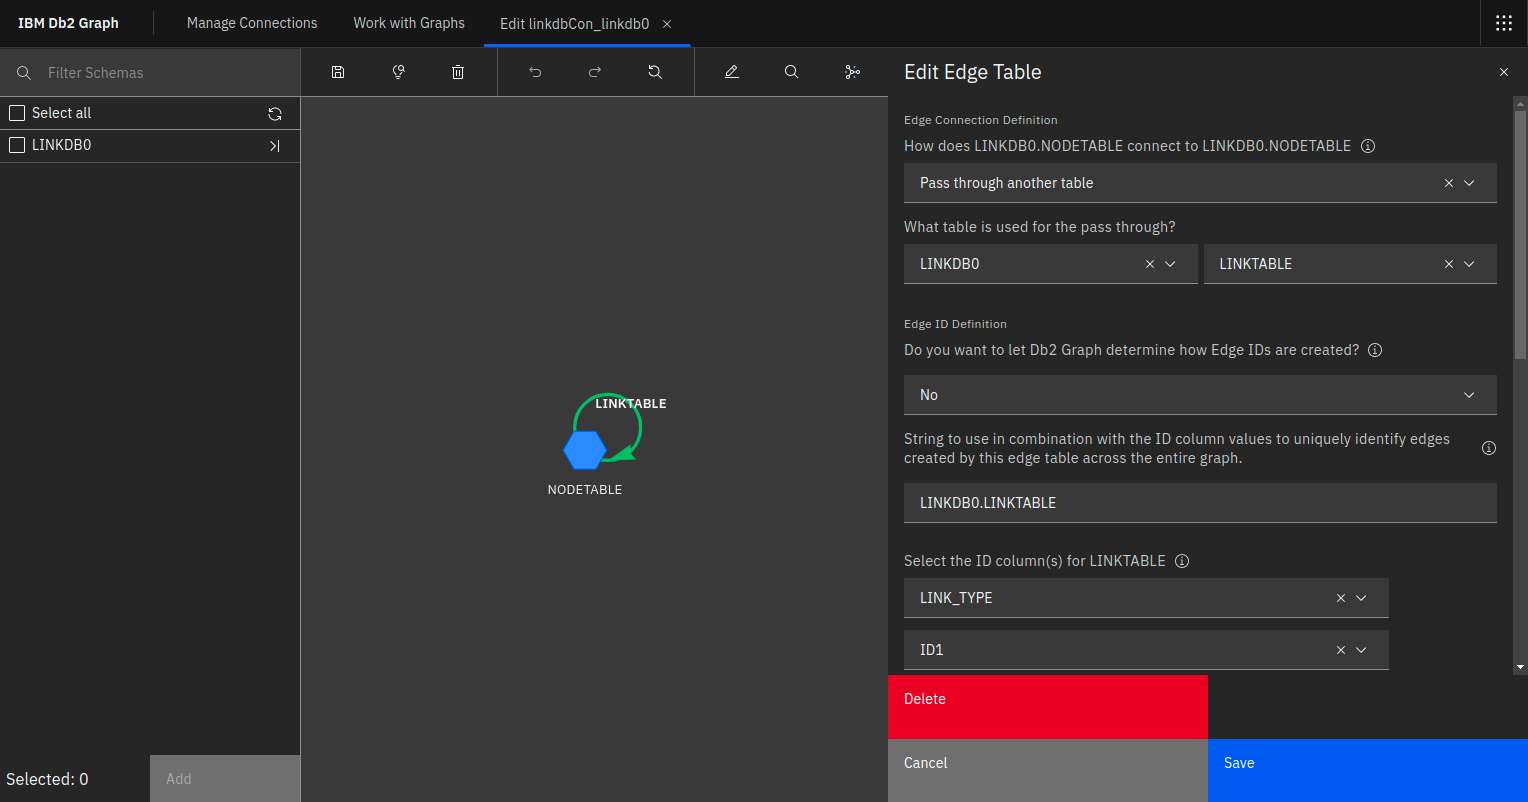
\includegraphics[width=\textwidth]{images/db2_graph_editor.png}
    \vspace{0.1em}
    \caption[Db2 Graph UI -- Graph-Modeler]{Db2 Graph UI -- Graph-Modeler zum Anlegen oder Editieren einer Graph-Overlay-Konfiguration}
    \label{fig:db2_graph_ui_editor}
\end{figure}

Für das Erstellen und Anlegen eines Graphen stellt Db2 Graph UI dabei auch einen sogenannten Graph-Modeler bereit \cite{ibm_docs_db2_graph_ui}. In diesem Graph-Modeler kann ein graphisches Modell eines Graphen angelegt und bearbeitet werden, dass diesen auch visuell abbildet. So kann beispielsweise eine Graph-Overlay mit einigen Klicks erstellt oder angepasst werden, siehe \autoref{fig:db2_graph_ui_editor}. Das in \autoref{fig:db2_graph_ui_editor} dargestellte Modell spiegelt dabei eine Konfiguration vergleichbar mit \autoref{src:mapping_example} wider. Die visuelle Darstellung bietet dabei den Vorteil, dass die Vertex-Tabellen und Edge-Tabellen sowie deren Zusammenspiel miteinander schneller erfasst werden können. Siehe das blaue Hexagon \texttt{NODETABLE}, welches eine Vertex-Tabelle repräsentiert oder den grünen Pfeil \texttt{LINKTABLE} der eine Edge-Tabelle abstrahiert in \autoref{fig:db2_graph_ui_editor}.

Zusätzlich zu dem Graph-Modeler bietet Db2 Graph UI auch eine Art Web-Console an \cite{ibm_docs_db2_graph_ui}. Diese wird auch als Query-Editor bezeichnet \cite{ibm_docs_db2_graph_ui}. Sie kann dabei dazu genutzt werden, Gremlin-Queries an Db2 Graph senden, ähnlich wie die Gremlin-Console. Die Web-Console setzt sich dabei allerdings durch ihre weiteren Funktionen von der Gremlin-Console ab. So besitzt die Web-Console auch die Fähigkeit, die abgefragten Elemente eines Graphen visuell darzustellen \cite{ibm_docs_db2_graph_ui}. Einerseits verschafft dies dem Nutzer einen Überblick über die Ergebnisse einer Gremlin-Query, siehe \autoref{fig:db2_graph_webconsole}. Anderseits bietet sie auch die Möglichkeit, mit der Ergebnismenge zu interagieren. Diese Interaktion ergibt sich daraus, dass sich abgebildete Knoten und Kanten auch anklicken und verschieben lassen.

\begin{figure}[ht]
    \centering
    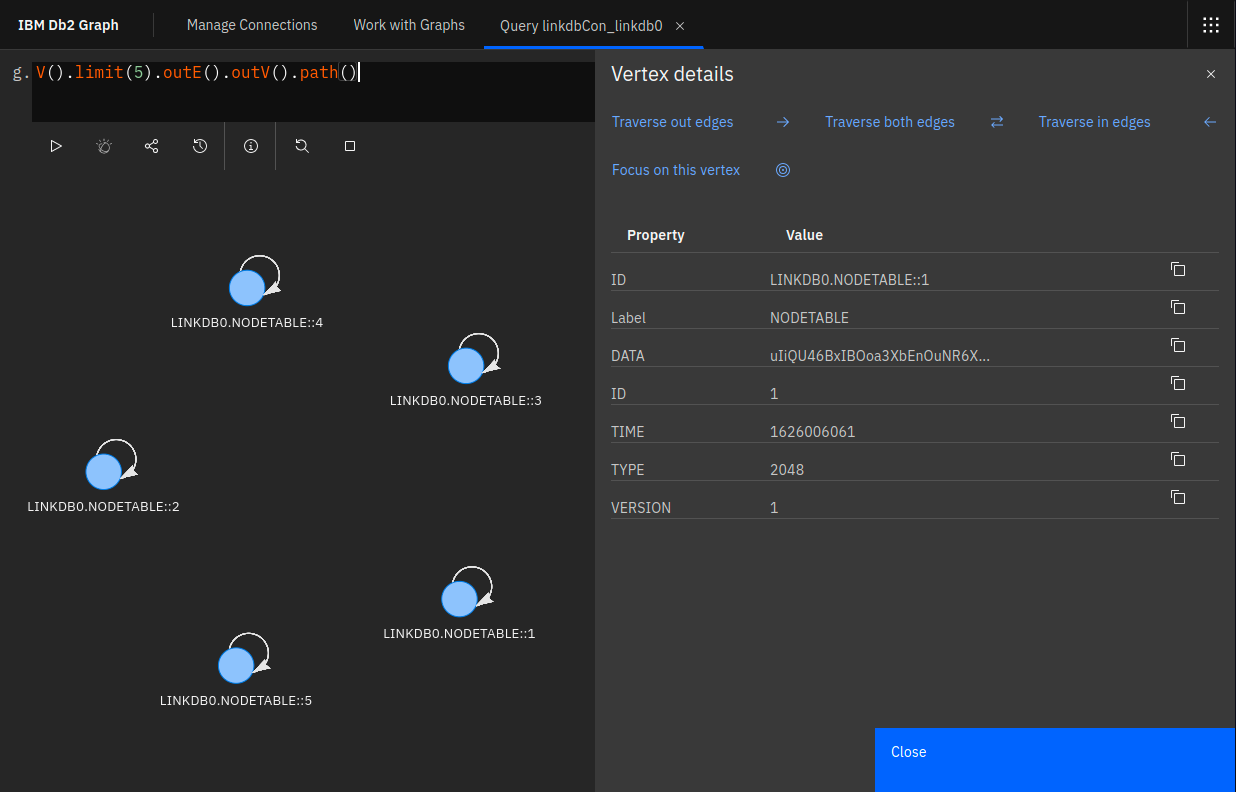
\includegraphics[width=\textwidth]{images/db2_graph_webconsole.png}
    \vspace{0.1em}
    \caption[Db2 Graph UI -- Web-Console]{Db2 Graph UI -- Web-Console}
    \label{fig:db2_graph_webconsole}
\end{figure}

Der bereits aus Beta 3 bekannte \texttt{manage}-Befehl ist, wie bereits zuvor angesprochen auch in V11.5.6.0 verfügbar \cite{ibm_docs_db2_graph_commands}. Allerdings wurde die Fähigkeiten des Befehls erheblich erweitert. So unterstützt er die neue Form des Session-Managements und Verbindungsaufbaus, die mit v11.5.6.0 in Db2 Graph eingeführt wurde \cite{ibm_docs_db2_graph_commands}. Während in Beta 3 die Interaktion mit Db2 Graph kaum Einschränkungen unterlag, erfordert beispielsweise das Anlegen eines Graphen folgende Schritte bei der Arbeit mit dem \texttt{manage}-Befehl:

\begin{enumerate}
    \item Das Öffnen einer Session -- hier \textit{linkdbS} genannt:\\
    \code{docker exec -it db2graph manage openSession linkdbS}
    \item Das erstmalige Erstellen einer Connection von Db2 Graph zu Db2 -- hier \textit{linkdbCon} genannt:\\
    \code{docker exec -it db2graph manage addConnection linkdbS linkdbCon 'Connection to db2 instance with linkdb0 database' localhost no 50000 linkdb0 db2inst1 linkdb}
    \item Das Öffenen der Connection -- hier die zuvor erstellte \textit{linkdbCon}:\\
    \code{docker exec -it db2graph manage openConnection linkdbS linkdbCon db2inst1 linkdb}
    \item Das Anlegen eines neuen Graphen für ein bestimmtes Datenbankschema -- hier \textit{linkdb0} als Graph und \textit{LINKDB0} als Datenbankschema:\\ 
    \code{docker exec -it db2graph manage addGraph linkdbS linkdbCon \break linkdb0 LINKDB0}
\end{enumerate}

Konträr zu diesem Ablauf musste bei Db2 Graph Beta 3 lediglich, der kurze Dialog der auf \code{docker exec -it db2graph manage add} folgte ausgefüllt werden. Darüber hinaus gilt es auch zu erwähnen, das Db2 Graph UI ebenfalls eine Connection anlegen und Öffnen muss, bevor ein Graph mit dem Graph-Modeler angelegt werden kann \cite{ibm_docs_db2_graph_ui}. Auf das Öffnen einer Session kann jedoch verzichtet werden, da dies von der Weboberfläche automatisch ohne Einbindung des Nutzers erfolgt.

Eine weitere Neuerung, die Einzug in V11.5.6.0 gehalten hat, stellt die Tatsache dar, dass das Graph-Modell eines angelegten Graphen immer auch in die Db2 Datenbank geschrieben wird \cite{ibm_docs_privileges}. Zuvor wurde die Mapping-Konfiguration ausschließlich in Db2 Graph gehalten. Db2 Graph V11.5.6.0 schreibt hingegen ein erstelltes Graph-Modell in die Tabelle \texttt{IBMGRAPH.IBMGRAPHMODEL} der Db2 Datenbank, welche die Vertex- und Edge-Tabellen des Graph-Modells beinhaltet. 

\subsection{Zusammenfassung}

Bei Db2 Graph handelt es sich um eine Graph-Erweiterung die genutzt werden kann, um Graph-Anfragen an eine relationale Datenbank zu stellen. 

Um diese Aufgabe zu erfüllen, nutzt sie eine Mapping-Konfiguration. Diese Mapping-Konfiguration beschreibt die Topologie eines Graphen. Dabei regelt sie, welche relationalen Tabellen Teil des Graphen sind und welche Rolle sie im Graphen einnehmen.

Anhand dieser Topologie Informationen und einer Gremlin-Query erzeugt Db2 Graph SQL-Code. Dieser wird anschließend an eine Db2 Instanz gesendet. Die im Anschluss daran von Db2 an Db2 Graph gesendete Ergebnismenge, wird schließlich von Db2 Graph aufbereitet und als Antwort auf die Gremlin-Query weitergegeben. 

Um als Graph-Erweiterung bei diesem Prozess eine möglichst hohe Performance und geringe Ressourcen Auslastung aufzuweisen, beherrscht Db2 Graph eine Vielzahl an Optimierungsmechanismen. 

Im Rahmen dieser Arbeit werden zwei verschiedene Versionen von Db2 Graph behandelt. Die ältere Variante Beta 3 und die neue Variante V11.5.6.0. Die beiden Versionen unterscheiden sich dabei hauptsächlich in den folgenden drei Punkten:

\begin{itemize}
    \item \textit{Optimierungstechniken}\\
    Die Optimierung von Db2 Graph ist in V11.5.6.0 weiter fortgeschritten als in Beta 3. 
    \item \textit{Usability}\\
    Die mit V11.5.6.0 eingeführte Db2 Graph UI erleichtert den Umgang und die Einrichtung von Db2 Graph erheblich. 
    \item \textit{Session- und Connection-Management}\\
    Das in V11.5.6.0 eingeführte Session- und Connection-Management verkompliziert die Interaktion mit Db2 Graph, im Vergleich zu Beta 3.
\end{itemize}